\documentclass[titlepage,11pt]{article}
\usepackage{comment}
\usepackage{enumitem}
\usepackage{transparent} % Untuk transparansi gambar
\usepackage{listings}
\usepackage{amsmath}
\usepackage{graphicx}
\usepackage[font=small,labelfont=bf]{caption}
\usepackage[bahasa]{babel}
\usepackage{float}
\usepackage{verbatim}
\usepackage{graphicx,tabularx,multirow}
\usepackage{xcolor}
\usepackage{subcaption}
\usepackage[onehalfspacing]{setspace}
\usepackage[
	allcolors=visigrey,
	colorlinks=true,
]{hyperref}
\usepackage[a4paper,left=2cm,right=2cm]{geometry}
% Pengaturan kutipan artikel
\usepackage[style=ieee, backend=biber]{biblatex}
%Code listing style pak akok
\definecolor{codegreen}{rgb}{0,0.6,0}
\definecolor{codegray}{rgb}{0.5,0.5,0.5}
\definecolor{codepurple}{rgb}{0.58,0,0.82}
\definecolor{backcolour}{rgb}{0.95,0.95,0.92}

\usepackage{eso-pic} % Untuk menambahkan elemen ke seluruh halaman

\newcommand\BackgroundPic{
  \put(0,0){
    \parbox[b][\paperheight]{\paperwidth}{
      \vfill
      \centering
      \transparent{0.1}
      
\includegraphics[width=0.4\paperwidth,keepaspectratio]{miot.png}
      \vfill
    }
  }
}

\newcommand\BackgroundAllPages{ \AddToShipoutPicture*{\BackgroundPic} }
\newcommand\BackgroundNone{ \ClearShipoutPicture } % hilangkan background

\lstdefinestyle{mystyle}{
	backgroundcolor=\color{backcolour}, commentstyle=\color{codegreen},
	keywordstyle=\color{magenta},
	numberstyle=\small\color{codegray},
	stringstyle=\color{codepurple},
	basicstyle=\ttfamily\footnotesize,
	breakatwhitespace=false,         
	breaklines=true,                 
	captionpos=t,                    
	keepspaces=true,                 
	numbers=left,                    
	numbersep=5pt,                  
	showspaces=false,                
	showstringspaces=false,
	showtabs=false,           
	frame = single,
	tabsize=2
}
\lstset{style=mystyle}

\definecolor{visigrey}{rgb}{.1,.15,.15}
\geometry{top=1cm,bottom=.5cm}
\savegeometry{titlepage}
\geometry{top=2cm,bottom=2cm}
\savegeometry{main}

\def\bspace{\(\qquad\qquad\qquad\)}
\usepackage[T1]{fontenc}
\usepackage[utf8]{inputenc}
\usepackage{tgheros}
\renewcommand*\familydefault{\sfdefault}

\setcounter{tocdepth}{6}

\def\autor{Laboratorium }
\def\lab{Multimedia dan Internet of Things}
\def\departemen{Departemen Teknik Komputer}
\def\institut{Institut Teknologi Sepuluh Nopember}
\def\praktikum{Laporan Akhir \\ Praktikum Jaringan Komputer}
\def\nama{Muhammad Zidane Faiq Sidqi - 5024231040}
% Ubah Judul sesuai dengan modul
\def\judul{Tunelling}
\def\tanggal{2025}
\begin{document}
% Ubah Bahasa sesuai dengan keinginan
\selectlanguage{bahasa}

\BackgroundNone
\def\headingtype{\bf \small}
\loadgeometry{titlepage}

\begin{titlepage}
	\centering
	\begin{tabularx}{\textwidth}{l@{\hskip 0pt}lX}
		\raisebox{-0.5\height}{
\includegraphics[width=3cm]{Cover/img/logodepart.png}} 
		& \raisebox{-0.5\height}{
\includegraphics[width=3cm]{Cover/img/miot.png}} 
		& \raggedleft
	\hfill
	\begin{minipage}{0.5\textwidth}
		\raggedleft
		{\emph{\headingtype \autor}} \\[-2pt]
		{\headingtype \lab} \\[-2pt]
		{\headingtype \departemen} \\[-2pt]
		{\headingtype \emph{\institut}}
	\end{minipage}

	\vspace{5cm}
	\end{tabularx}
	
	\vspace{5cm}
	{\Huge \bf \praktikum \par}
	
	\vspace{2cm}
	{\LARGE \bf \judul \par}
	
	\vspace{2cm}
	{\Large \nama \par}
	
	\vfill
	{\Large \tanggal \par}
	
	\vfill
	
\includegraphics[width=\textwidth]{Cover/img/footer.png}
\end{titlepage}

\loadgeometry{main}


\BackgroundAllPages
% Pilih Modul yang akan di build
\section{Langkah-Langkah Percobaan}
\subsection{Konfigurasi Router VPN PPTP PC dengan Router}
1. Konfigurasi DHCP Client (Koneksi Internet).
\begin{figure}[H]
    \centering
    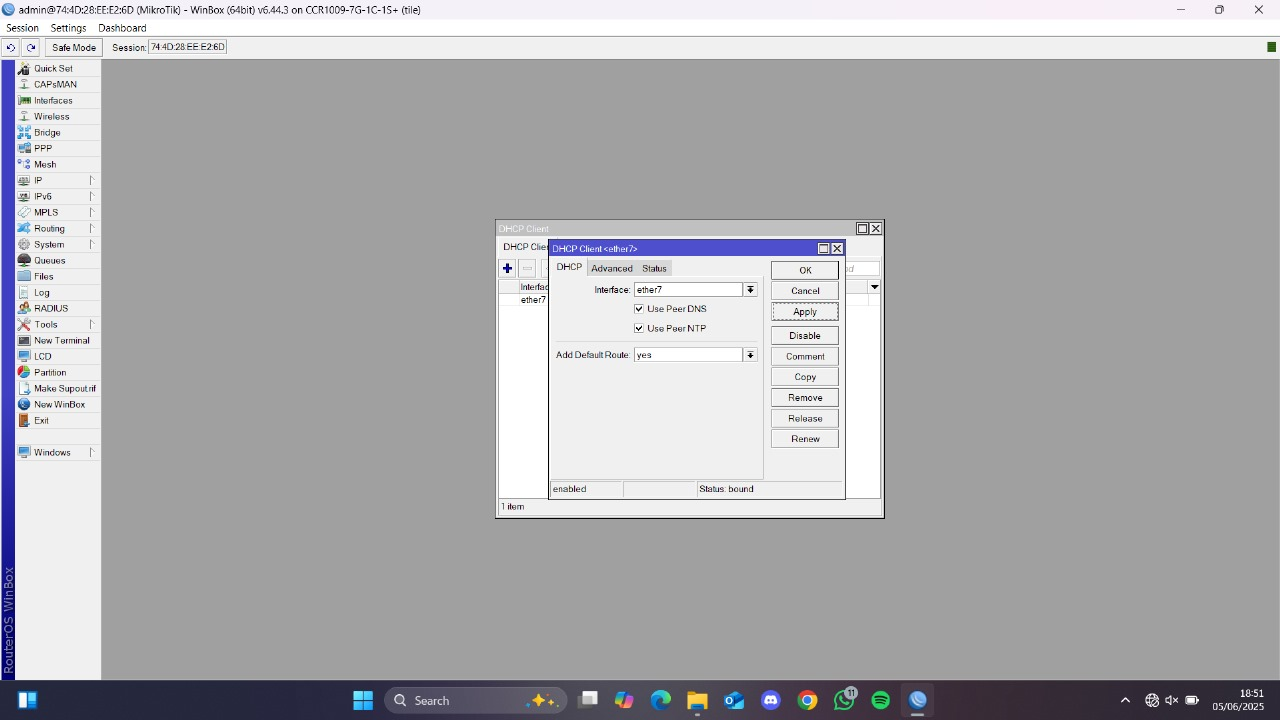
\includegraphics[width=0.65\linewidth]{image/tun4.jpg}
    \label{fig:inirujukan}
    \caption{Konfigurasi DHCP client}
\end{figure}
2. Konfigurasi Firewall NAT.
\begin{figure}[H]
    \centering
    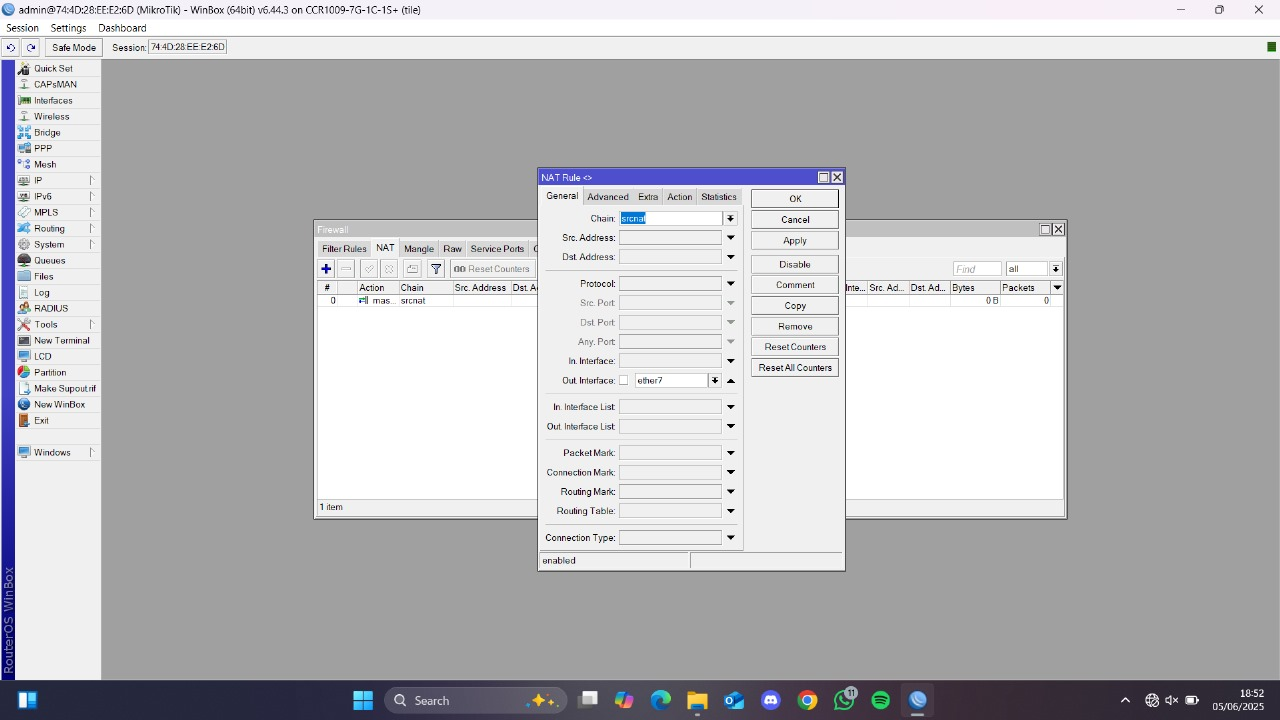
\includegraphics[width=0.65\linewidth]{image/tun5.jpg}
    \label{fig:inirujukan}
\end{figure}
\begin{figure}[H]
    \centering
    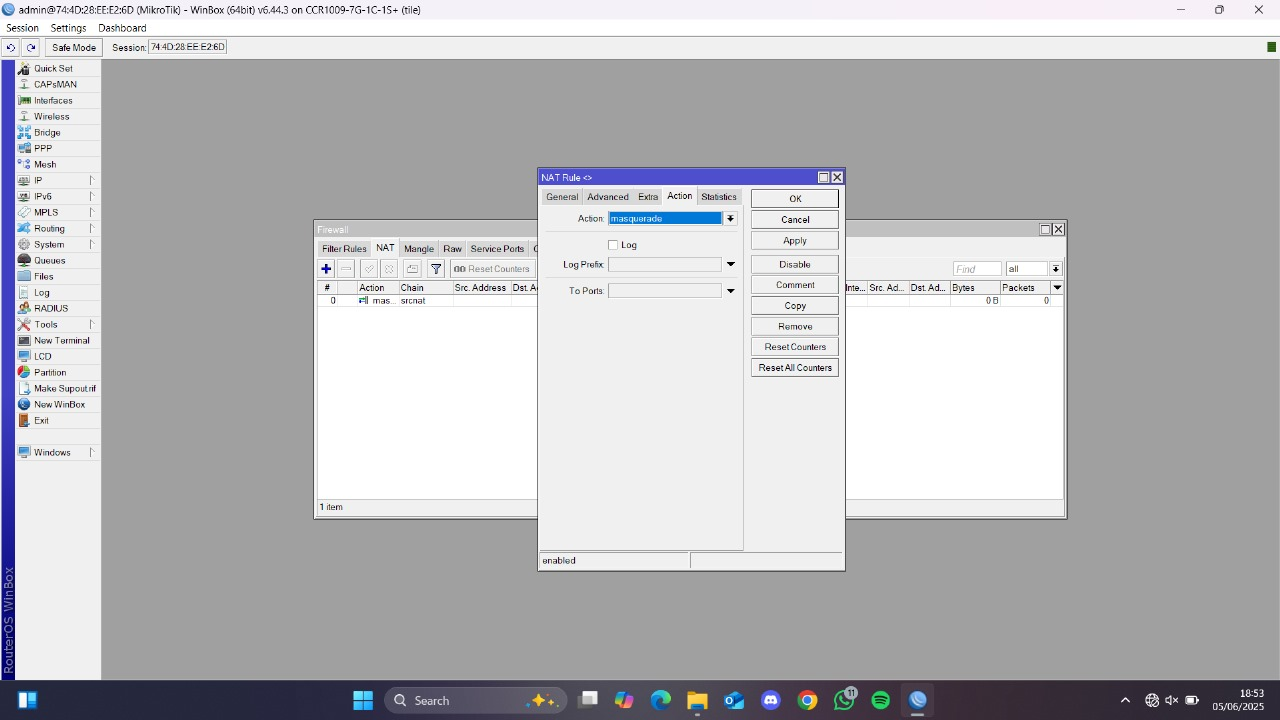
\includegraphics[width=0.65\linewidth]{image/tun6.jpg}
    \label{fig:inirujukan}
    \caption{Konfigurasi NAT}
\end{figure}
3. Konfigurasi Alamat IP Lokal (LAN).
\begin{figure}[H]
    \centering
    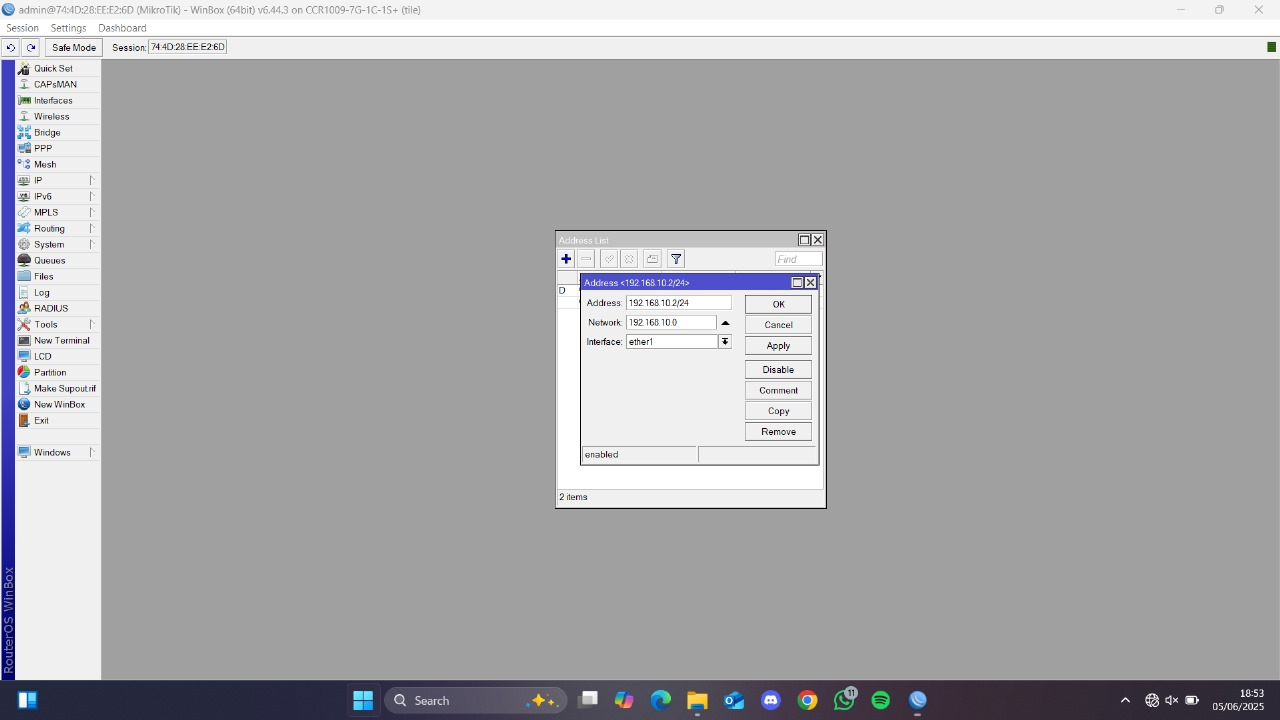
\includegraphics[width=0.65\linewidth]{image/tun7.jpg}
    \label{fig:inirujukan}
    \caption{Konfigurasi IP lokal}
\end{figure}
4. Konfigurasi DHCP Server (Distribusi IP ke Klien) Atur server DHCP agar perangkat klien (laptop/PC) yang terhubung ke ether1 mendapatkan IP secara otomatis.
\begin{figure}[H]
    \centering
    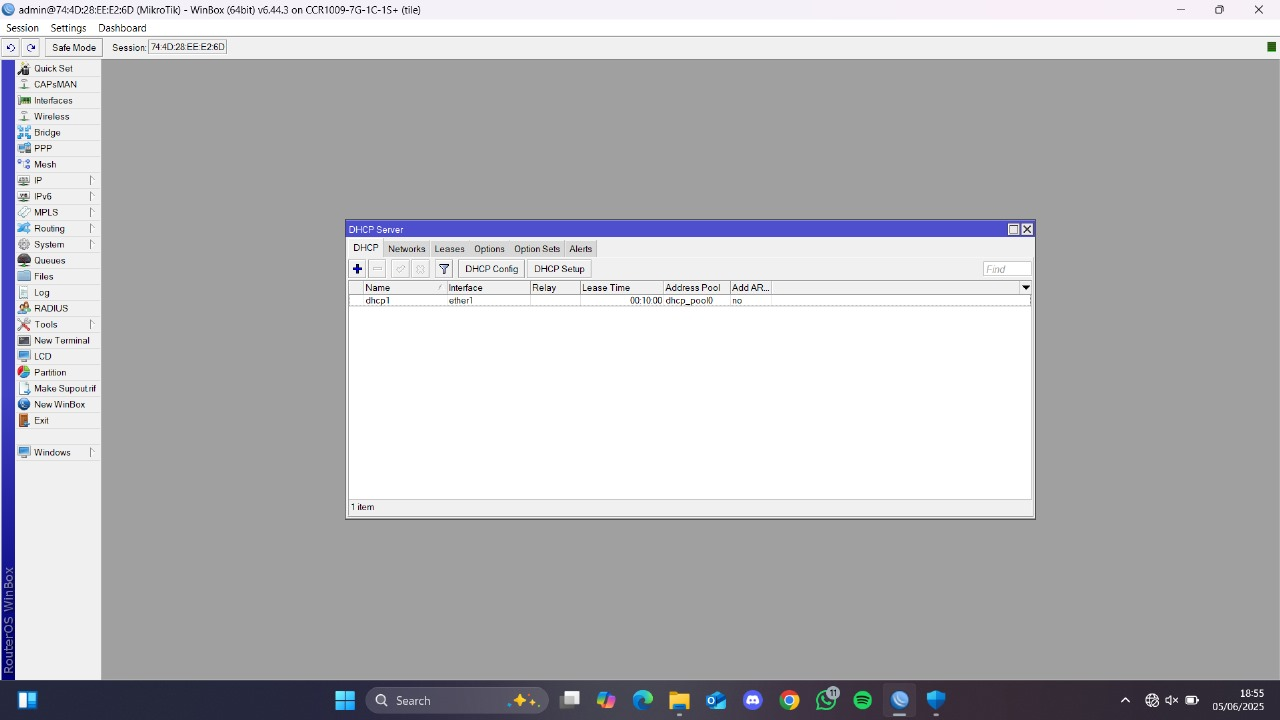
\includegraphics[width=0.65\linewidth]{image/tun8.jpg}
    \label{fig:inirujukan}
    \caption{Konfigurasi DHCP server}
\end{figure}
5. Mengaktifkan Proxy ARP Ubah mode ARP pada interface yang terhubung ke PC2 untuk membantu proses bridging dan routing.
\begin{figure}[H]
    \centering
    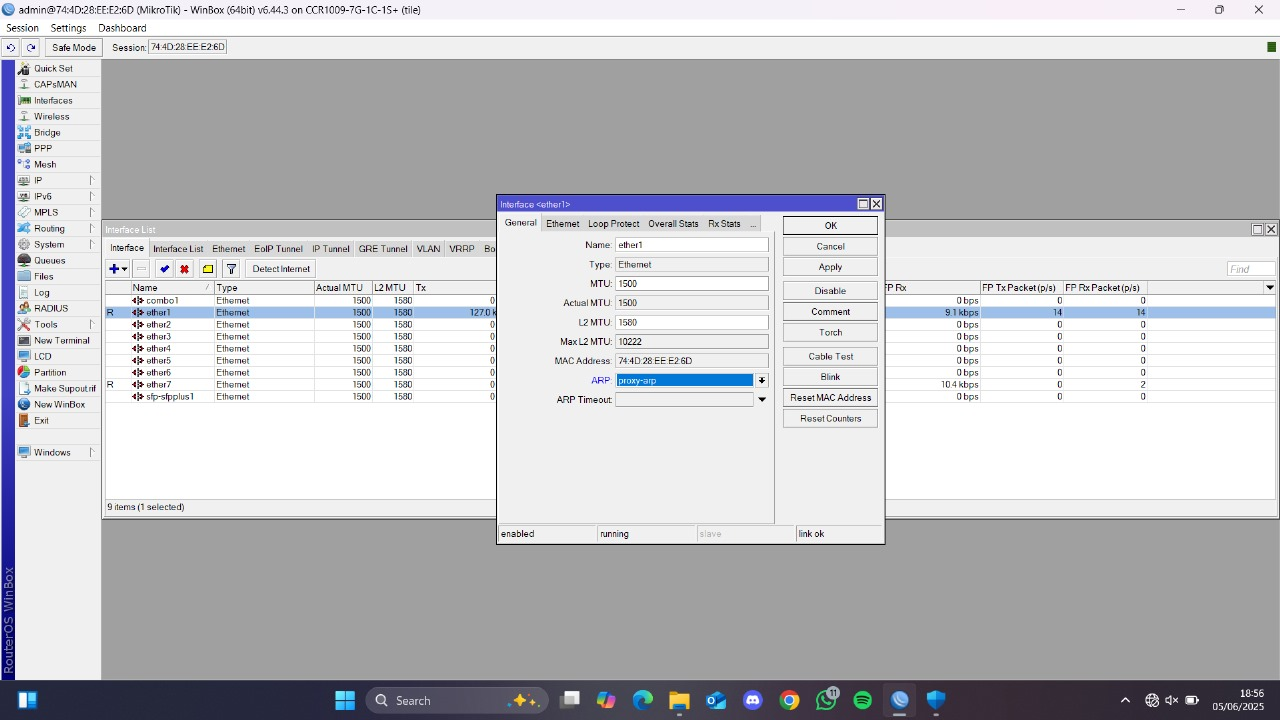
\includegraphics[width=0.65\linewidth]{image/tun9.jpg}
    \label{fig:inirujukan}
    \caption{Proxy ARP aktif}
\end{figure}
6. Konfigurasi PPTP Server VPN. \\ 
a. Mengaktifkan PPTP Server
\begin{figure}[H]
    \centering
    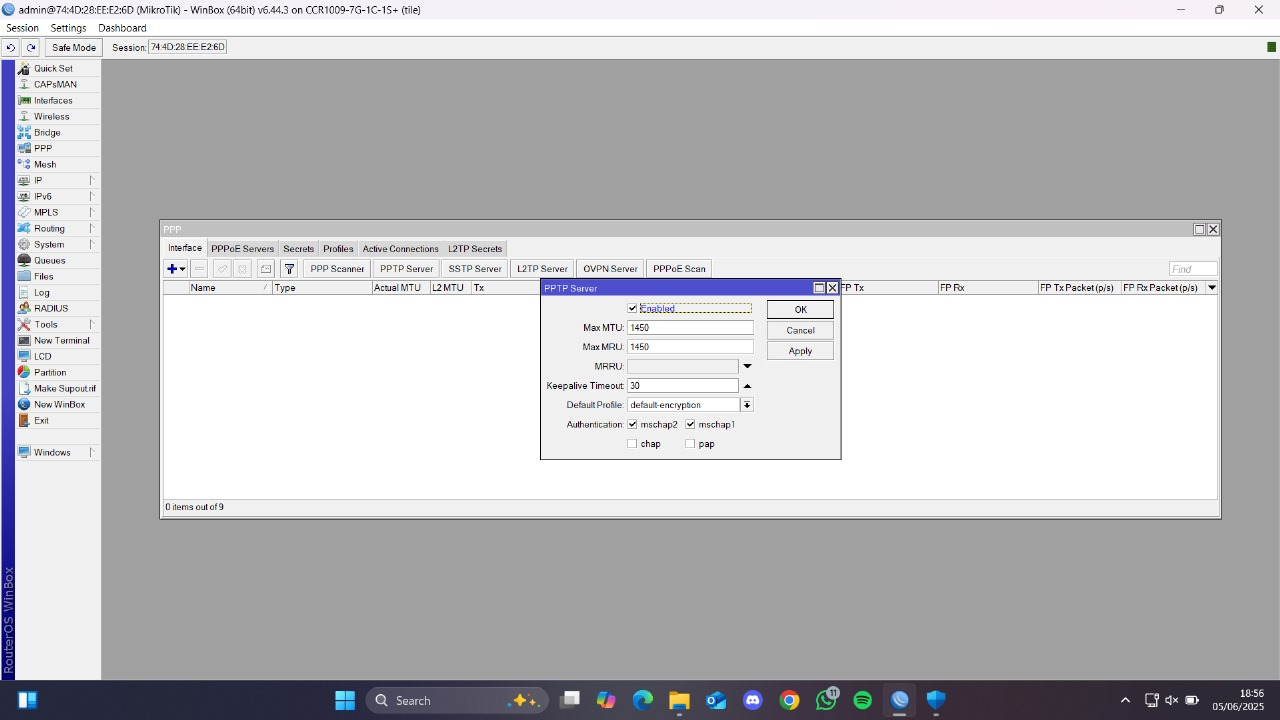
\includegraphics[width=0.65\linewidth]{image/tun10.jpg}
    \label{fig:inirujukan}
    \caption{Konfiguras PPTP server}
\end{figure}
b. Membuat User dan Password (Secrets) Kredensial ini akan digunakan oleh klien untuk login VPN.
\begin{figure}[H]
    \centering
    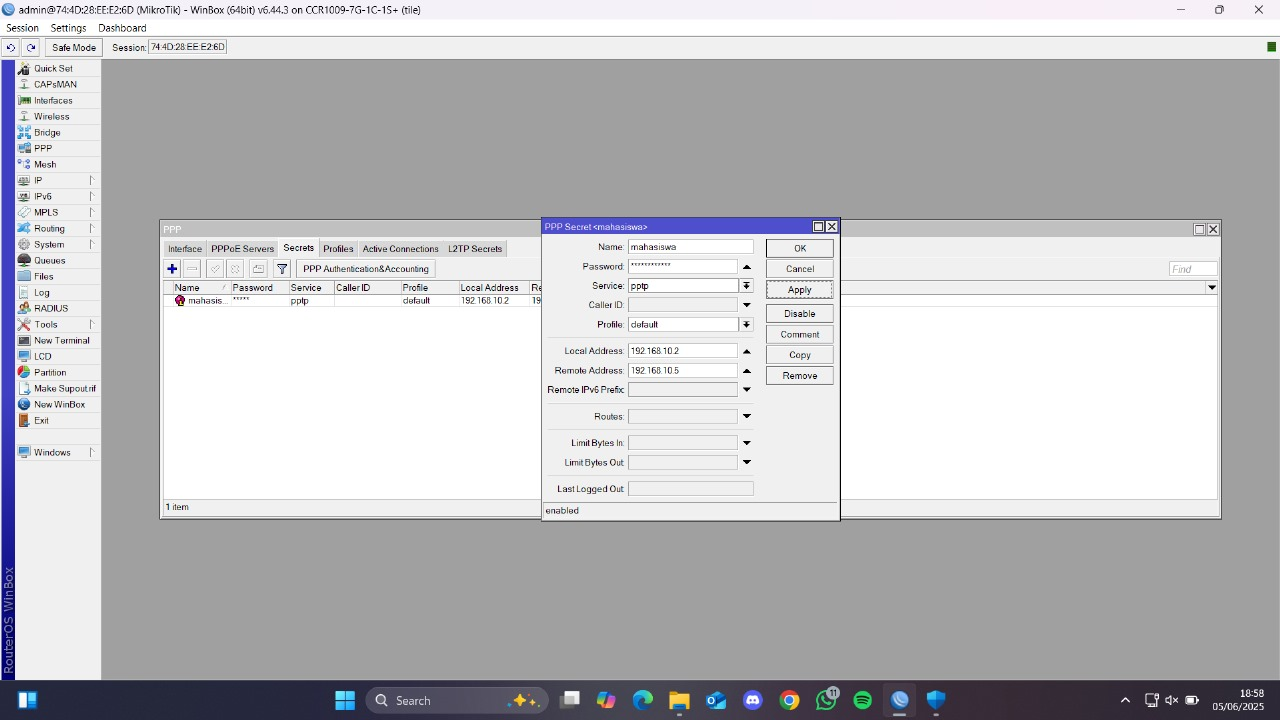
\includegraphics[width=0.65\linewidth]{image/tun11.jpg}
    \label{fig:inirujukan}
    \caption{Pembuatan user dan password}
\end{figure}
7. Konfigurasi PPTP Client di Laptop (Windows). 
\begin{figure}[H]
    \centering
    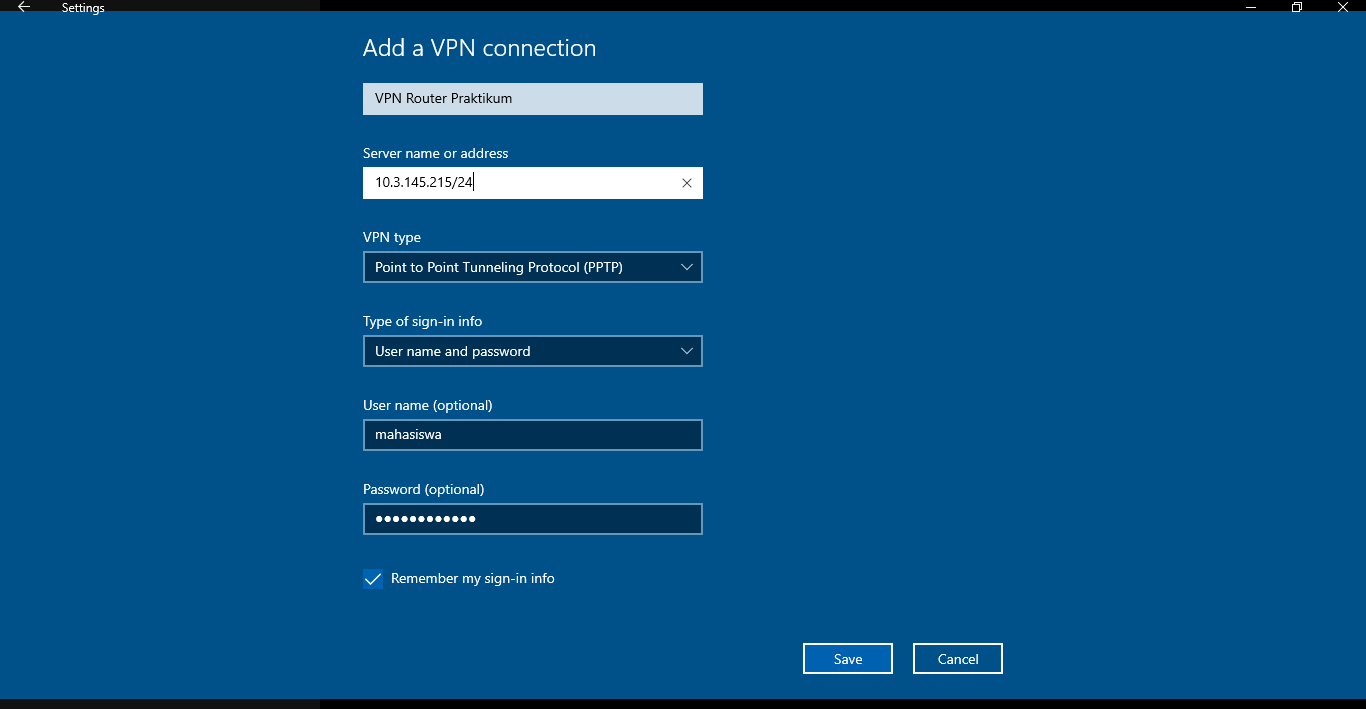
\includegraphics[width=0.65\linewidth]{image/tun1.png}
    \label{fig:inirujukan}
\end{figure}
\begin{figure}[H]
    \centering
    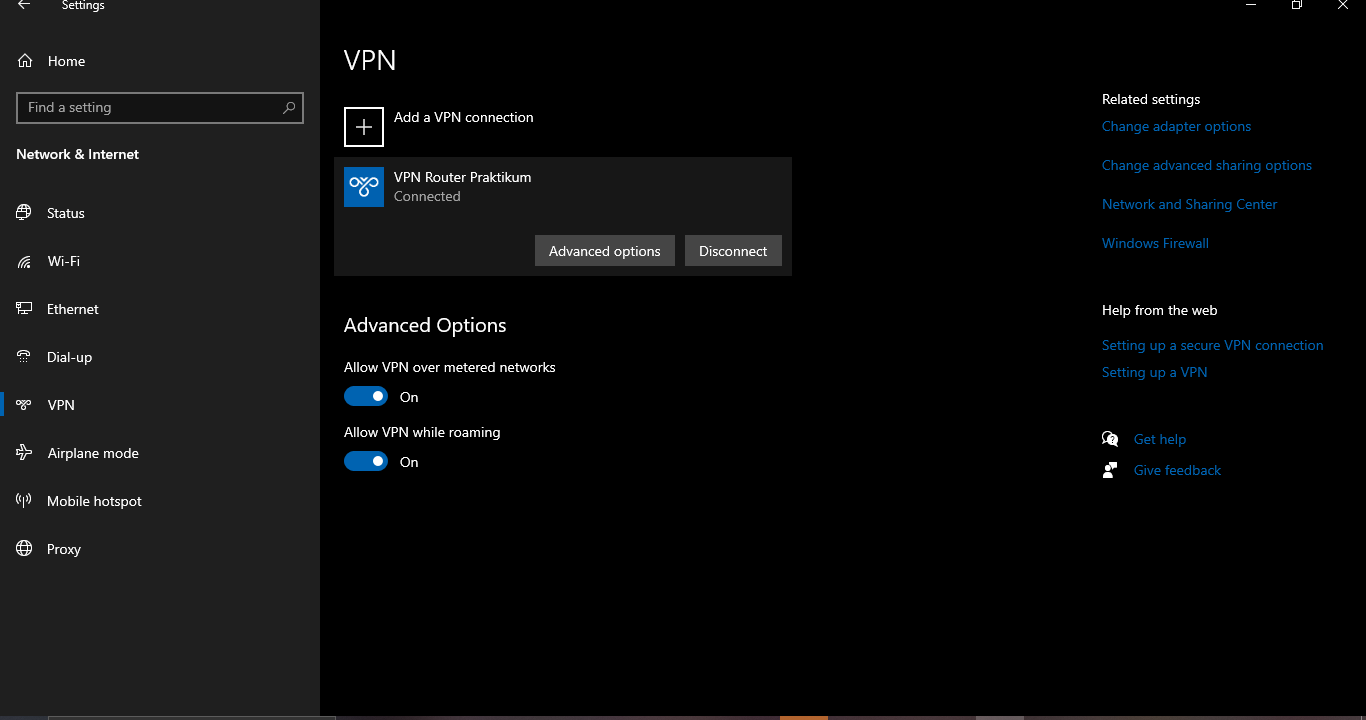
\includegraphics[width=0.65\linewidth]{image/tun2.png}
    \label{fig:inirujukan}
    \caption{Konfigurasi PPTP client}
\end{figure}
8. Verifikasi dan Pengujian. \\
a. Verifikasi di PC 1 yang terhubung VPN dan ping 192.168.10.2.
\begin{figure}[H]
    \centering
    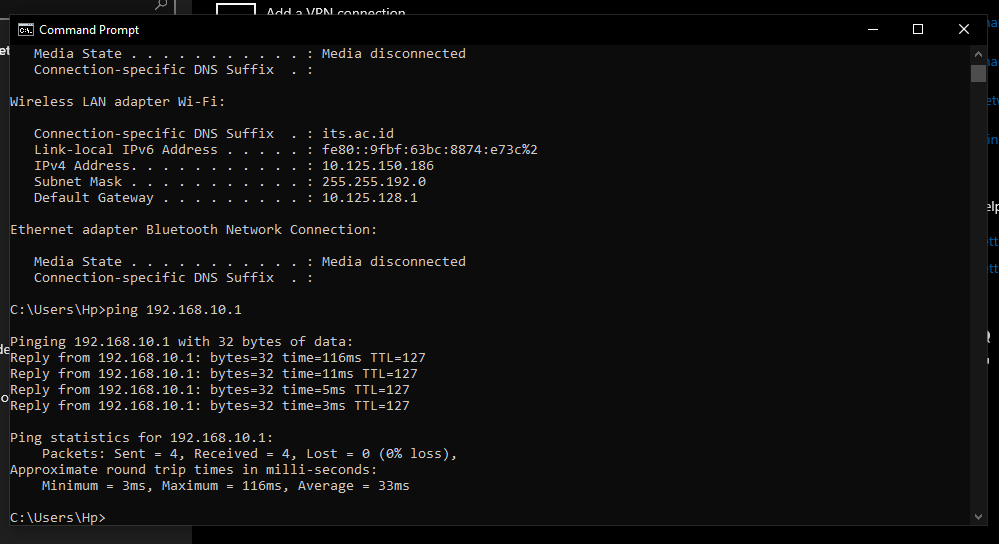
\includegraphics[width=0.65\linewidth]{image/tun3.png}
    \label{fig:inirujukan}
    \caption{cmd pada pc1}
\end{figure}
b. Verifikasi di PC 2 (Yang terhubung ke ether1) dan uji ping pc.
\begin{figure}[H]
    \centering
    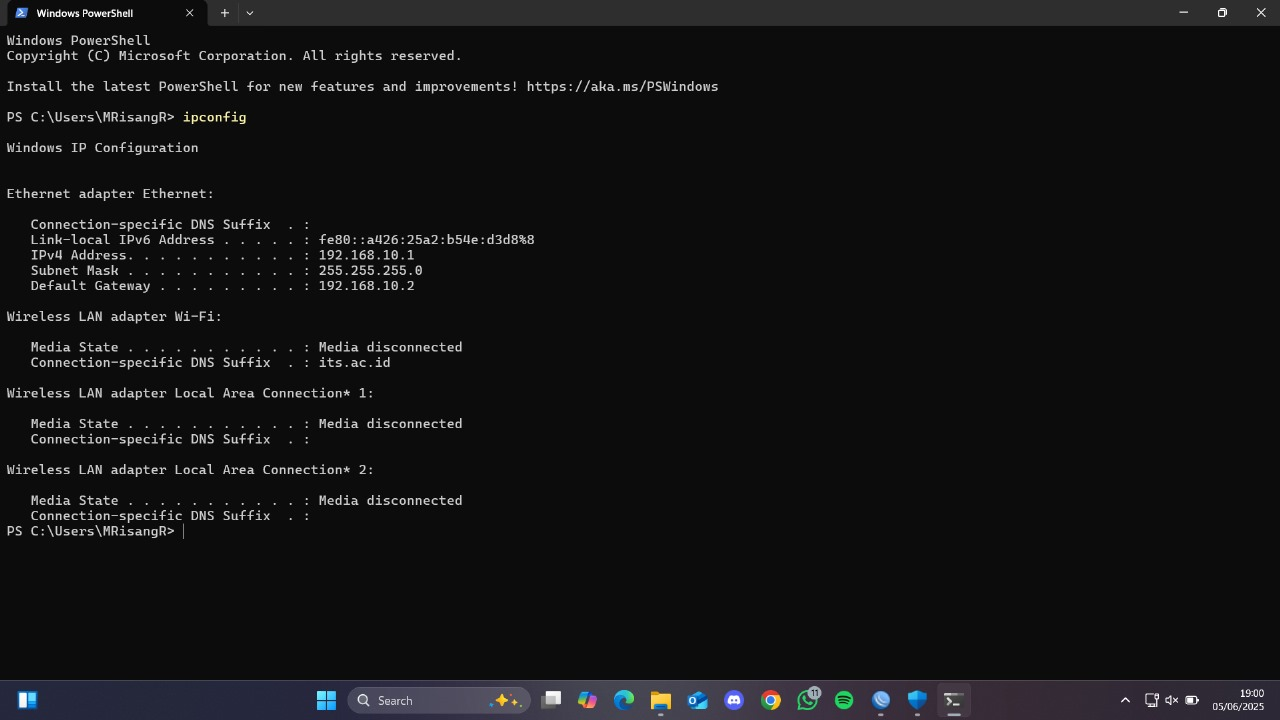
\includegraphics[width=0.65\linewidth]{image/tun16.jpg}
    \label{fig:inirujukan}
    \caption{tcmd pada pc2}
\end{figure}
\subsection{Konfigurasi QOS PC dengan Router}
1. Membuat Aturan Simple Queue Langkah ini bertujuan untuk membatasi kecepatan upload dan download untuk klien yang terhubung ke jaringan. 
\begin{figure}[H]
    \centering
    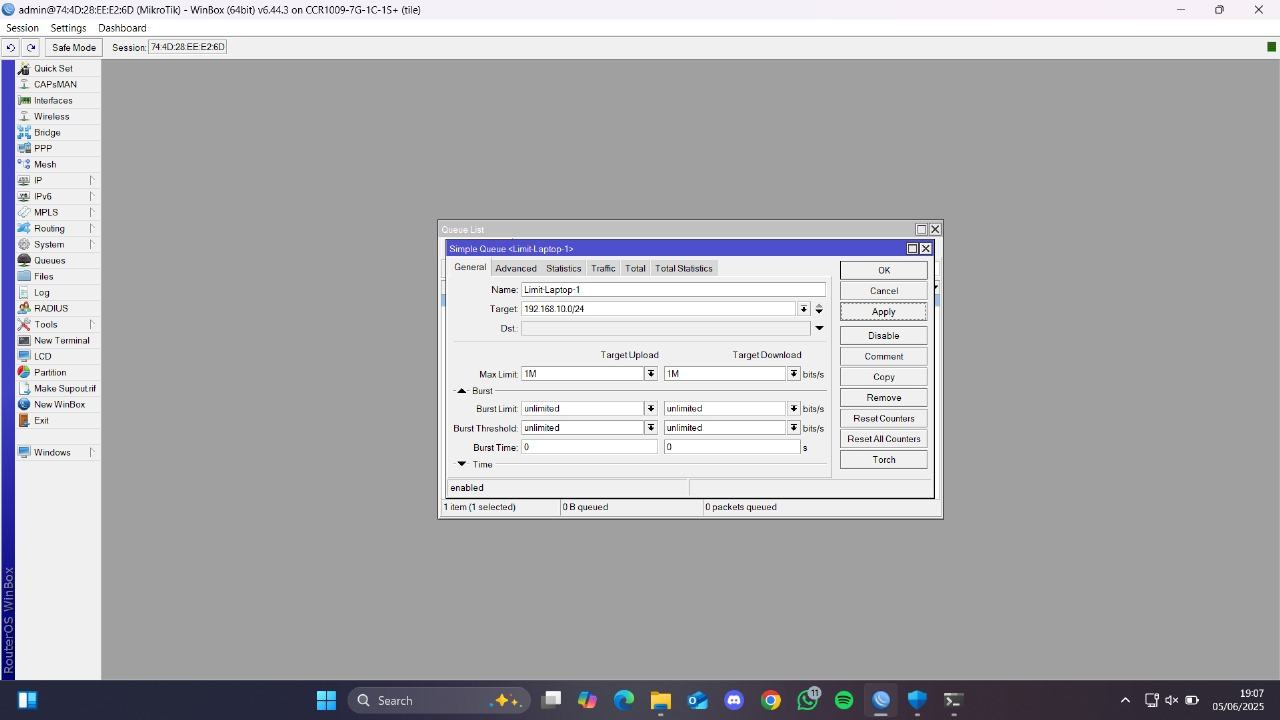
\includegraphics[width=0.65\linewidth]{image/tun12.jpg}
    \label{fig:inirujukan}
\end{figure}
2. Memantau Penggunaan Traffic.
\begin{figure}[H]
    \centering
    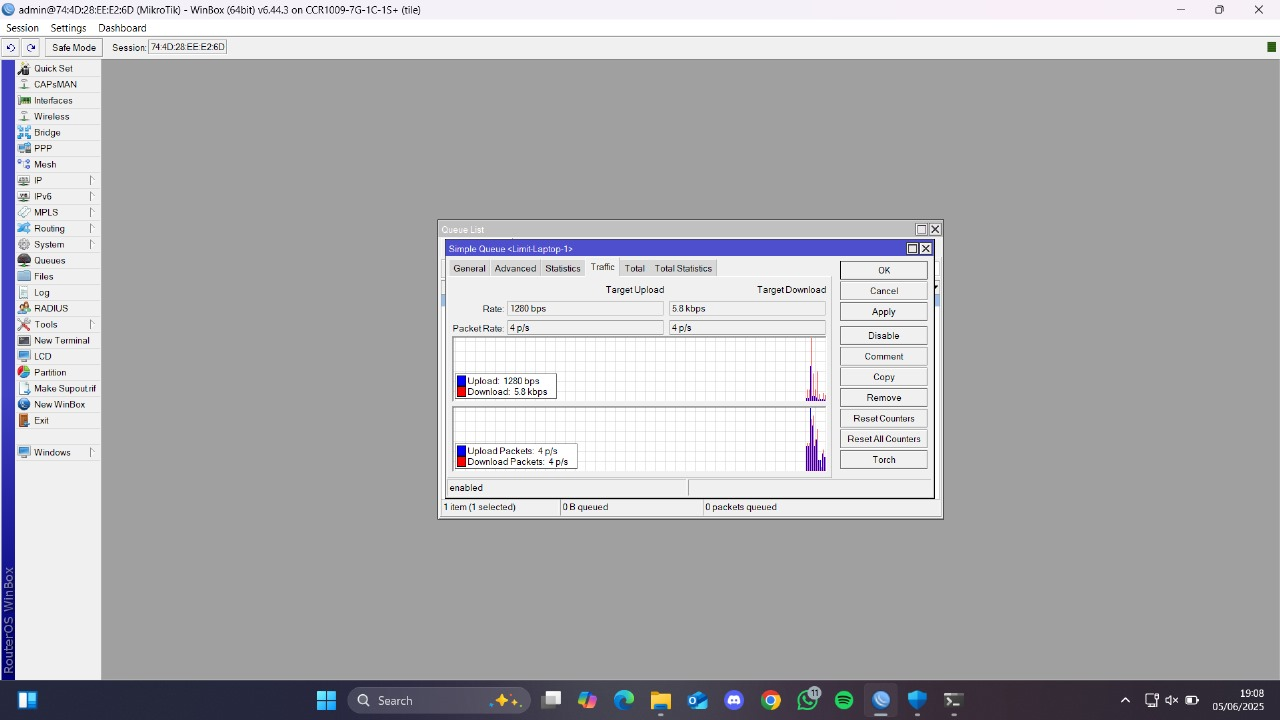
\includegraphics[width=0.65\linewidth]{image/tun13.jpg}
    \label{fig:inirujukan}
\end{figure}
3. Pengujian Efektivitas Queue. \\
a. Tes Saat Queue Tidak Aktif.
\begin{figure}[H]
    \centering
    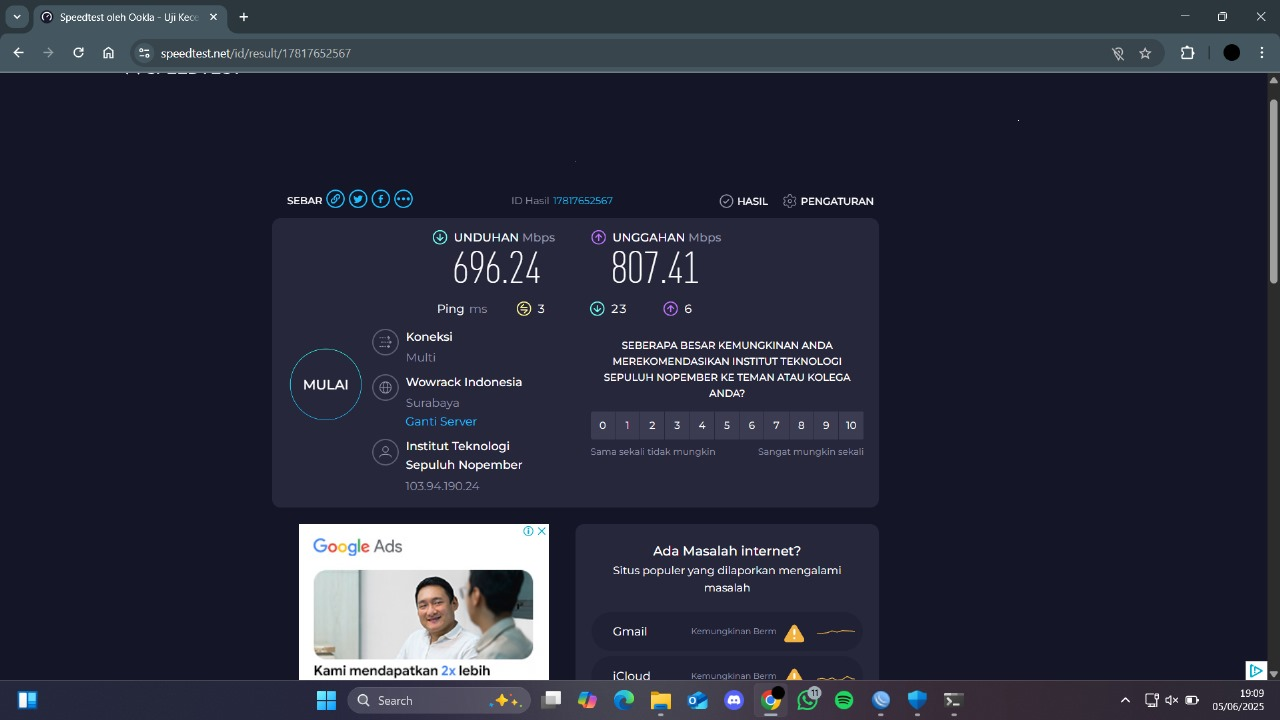
\includegraphics[width=0.65\linewidth]{image/tun14.jpg}
    \label{fig:inirujukan}
\end{figure}
b. Tes Saat Queue Aktif.
\begin{figure}[H]
    \centering
    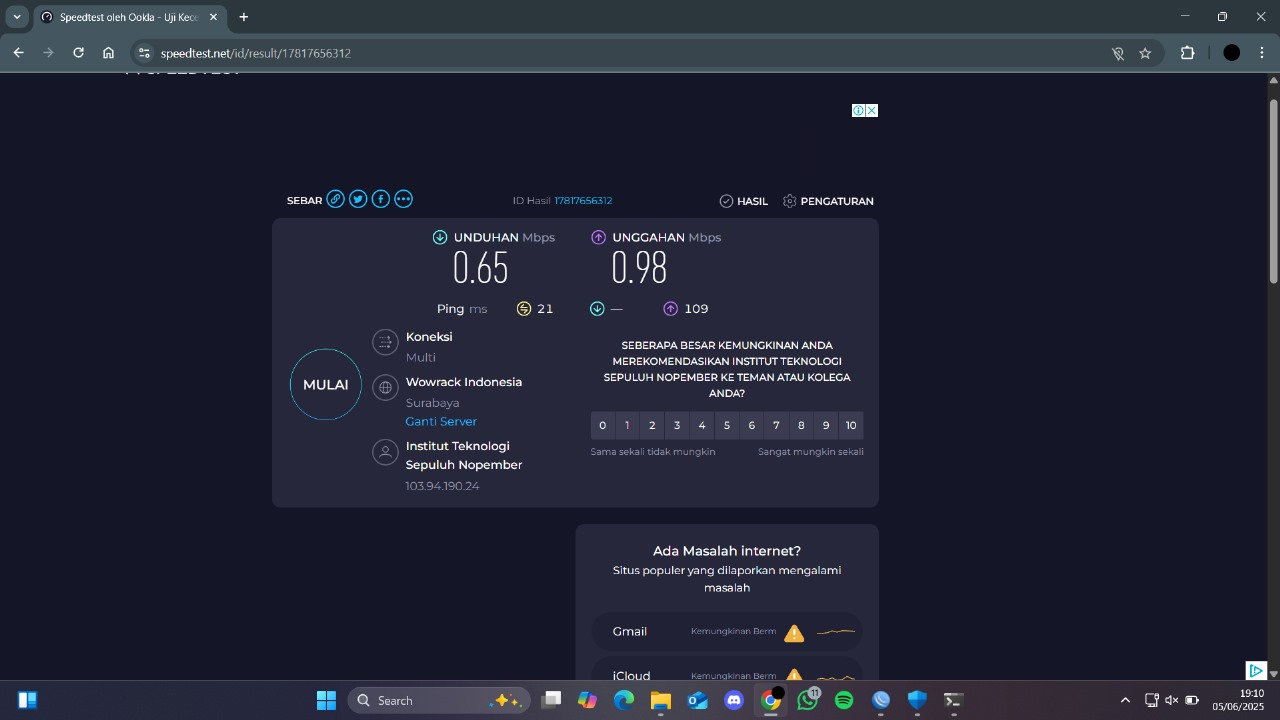
\includegraphics[width=0.65\linewidth]{image/tun15.jpg}
    \label{fig:inirujukan}
\end{figure}

\section{Analisis Hasil Percobaan}
Analisis hasil percobaan pada modul ini berfokus pada dua aspek utama: konfigurasi VPN PPTP dan implementasi Simple Queue untuk manajemen bandwidth. Pada percobaan konfigurasi VPN PPTP, langkah-langkah yang dilakukan meliputi reset konfigurasi router, pengaturan DHCP Client untuk koneksi internet, konfigurasi Firewall NAT, penetapan alamat IP lokal pada interface LAN, konfigurasi DHCP Server, pengaktifan Proxy ARP, serta pengaturan PPTP Server dan pembuatan user VPN. Hasil percobaan menunjukkan keberhasilan dalam membangun koneksi VPN PPTP antara router dan client (laptop Windows). \\ Secara teoritis, PPTP adalah salah satu protokol tunneling VPN yang membungkus paket IP dengan header tambahan dan mengirimkannya melalui "terowongan". Meskipun merupakan salah satu protokol VPN paling awal dan sudah banyak digunakan, PPTP memiliki kekurangan dalam hal keamanan dibandingkan protokol seperti IPSec karena tidak menyediakan enkripsi secara built-in dan rentan terhadap serangan tertentu. Namun, dalam konteks percobaan ini yang bertujuan untuk membangun konektivitas dasar, PPTP efektif dalam menciptakan "terowongan digital" agar data dari satu jaringan dapat terhubung ke jaringan lain yang berbeda jenis. \\ Verifikasi dan pengujian dilakukan dengan ipconfig pada CMD untuk memeriksa interface PPP baru dan melakukan ping ke alamat IP lokal router dan PC lain yang terhubung ke router. Hasil ping yang berhasil menunjukkan bahwa konektivitas melalui tunnel PPTP telah terbentuk dengan baik, memungkinkan komunikasi antar jaringan yang terpisah secara fisik. Tidak ada kesalahan alat atau langkah percobaan yang signifikan diidentifikasi yang memengaruhi hasil konfigurasi PPTP. \\ Percobaan kedua melibatkan konfigurasi Simple Queue untuk manajemen bandwidth. Langkah-langkah yang dilakukan adalah membuat aturan Simple Queue dengan batasan upload dan download sebesar 1 Mbps untuk seluruh network client (192.168.10.0/24). Pemantauan traffic dilakukan melalui tab "Traffic" pada Winbox, dan pengujian efektivitas queue dilakukan dengan membandingkan kecepatan internet sebelum (saat queue dinonaktifkan) dan sesudah (saat queue diaktifkan) aturan diterapkan menggunakan speedtest.net. \\ Perbandingan hasil percobaan dengan teori menunjukkan kesesuaian. Simple Queue memang dirancang untuk membatasi bandwidth secara langsung pada target IP atau network tertentu. Tidak ada kesalahan alat atau langkah percobaan yang signifikan yang mengganggu fungsionalitas Simple Queue. Keberhasilan dalam membatasi bandwidth ini menunjukkan pemahaman praktikan terhadap konsep manajemen bandwidth dasar menggunakan Simple Queue

\section{Hasil Tugas Modul}
\begin{figure}[H]
    \centering
    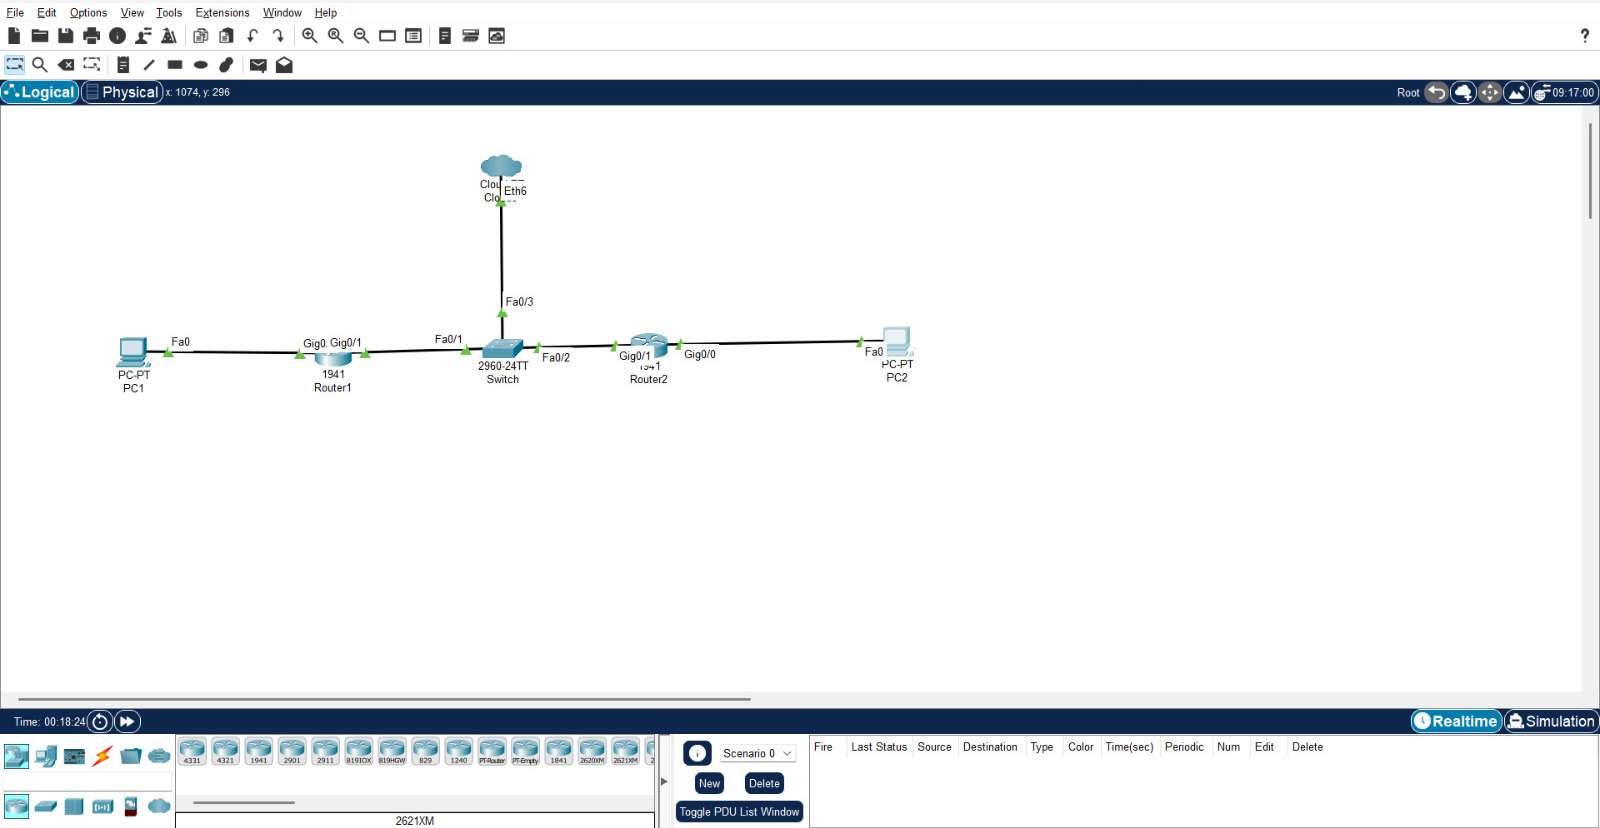
\includegraphics[width=0.65\linewidth]{image/tumod.jpg}
    \label{fig:inirujukan}
    \caption{hasil tugas modul}
\end{figure}
\begin{figure}[H]
    \centering
    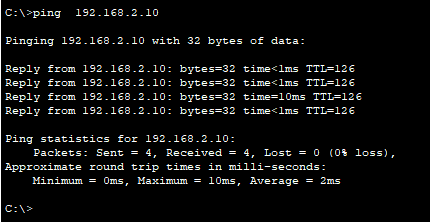
\includegraphics[width=0.65\linewidth]{image/tumod1.png}
    \label{fig:inirujukan}
    \caption{ping pc1 ke pc2}
\end{figure}
\subsection {Konfigurasi Ip address} 
- PC 1 : 192.168.1.10/24 \\
- PC 2 : 192.168.2.10/24 \\
- router 1 : 192.168.1.1/24 ; 10.0.0.1/24 \\
- router 2 : 192.168.2.1/24 ; 10.0.0.2/24
\subsection{Konfigurasi Tunnel}
\# Router 1 : \\ 
Router1(config)\#interface Tunnel0 \\
Router1(config-if)\#ip address 172.16.1.1 255.255.255.252 \\
Router1(config-if)\#tunnel source GigabitEthernet0/1 \\
Router1(config-if)\#tunnel destination 10.0.0.2 \\
Router1(config-if)\#tunnel mode gre ip \\
Router1(config-if)\#exit \\
Router1(config)\#ip route 192.168.2.0 255.255.255.0 Tunnel0. \\
\# Router 2 : \\
Router2(config)\#interface Tunnel0 \\
Router2(config-if)\#ip address 172.16.1.2 255.255.255.252 \\
Router2(config-if)\#tunnel source GigabitEthernet0/1 \\
Router2(config-if)\#tunnel destination 10.0.0.1 \\
Router2(config-if)\#tunnel mode gre ip \\
Router2(config-if)\#exit \\ 
Router2(config)\#ip route 192.168.1.0 255.255.255.0 Tunnel0.
\subsection{Penjelasan PPTP}
PPTP menciptakan koneksi virtual (terowongan) di atas Internet. Lalu lintas data dari jaringan PC1 menuju jaringan PC2 akan dienkapsulasi dan mungkin dienkripsi (tergantung implementasi dan konfigurasi) oleh PPTP saat melewati terowongan ini. Dengan PPTP, seolah-olah ada "kabel virtual" yang membentang dari Router 1 ke Router 2. Ini memungkinkan PC1 untuk berkomunikasi langsung dengan PC2 (misalnya, melakukan ping) seolah-olah mereka berada di jaringan yang sama atau terhubung langsung, meskipun lalu lintas fisiknya melewati internet. \\ Singkatnya, PPTP berfungsi sebagai jembatan virtual yang aman dan terenkapsulasi yang menghubungkan dua jaringan lokal yang terpisah secara fisik melalui jaringan publik (Internet), memungkinkan komunikasi transparan antara perangkat di kedua sisi jaringan seolah-olah mereka berada dalam satu jaringan pribadi yang besar. Ini adalah cara untuk menciptakan koneksi site-to-site VPN.
\section{Kesimpulan}
Berdasarkan hasil praktikum yang telah dilakukan, dapat disimpulkan beberapa hal penting terkait konfigurasi VPN PPTP dan manajemen bandwidth menggunakan Simple Queue pada router MikroTik. Tujuan praktikum, yaitu membangun koneksi aman antar jaringan menggunakan VPN PPTP dan mengimplementasikan manajemen bandwidth, telah berhasil dicapai. \\ Praktikum berhasil membangun koneksi VPN site-to-site (walaupun dalam simulasi adalah remote access antara router dan PC) menggunakan protokol PPTP. Implementasi Simple Queue juga berhasil dilakukan untuk membatasi kecepatan upload dan download pada client. Pengujian kecepatan internet sebelum dan sesudah penerapan Simple Queue menunjukkan bahwa bandwidth client berhasil dibatasi sesuai dengan konfigurasi yang ditetapkan. \\ Praktikum memberikan pemahaman mendalam tentang konsep tunneling dan peran VPN dalam menciptakan koneksi aman antar jaringan. Praktikan belajar bagaimana mengontrol dan mengalokasikan bandwidth menggunakan fitur Simple Queue pada MikroTik. Praktikum ini mengasah keterampilan konfigurasi router MikroTik, mulai dari pengaturan dasar seperti DHCP dan NAT hingga konfigurasi layanan yang lebih kompleks seperti VPN dan QoS. Pentingnya verifikasi setiap tahapan konfigurasi dengan alat seperti ping dan speedtest ditekankan dalam praktikum. \\ Secara keseluruhan, praktikum ini berhasil memberikan pengalaman langsung dalam mengimplementasikan konsep-konsep jaringan esensial, seperti VPN dan manajemen bandwidth, yang sangat relevan dalam dunia industri dan teknologi informasi.

\section{Lampiran}
\begin{figure}[H]
    \centering
    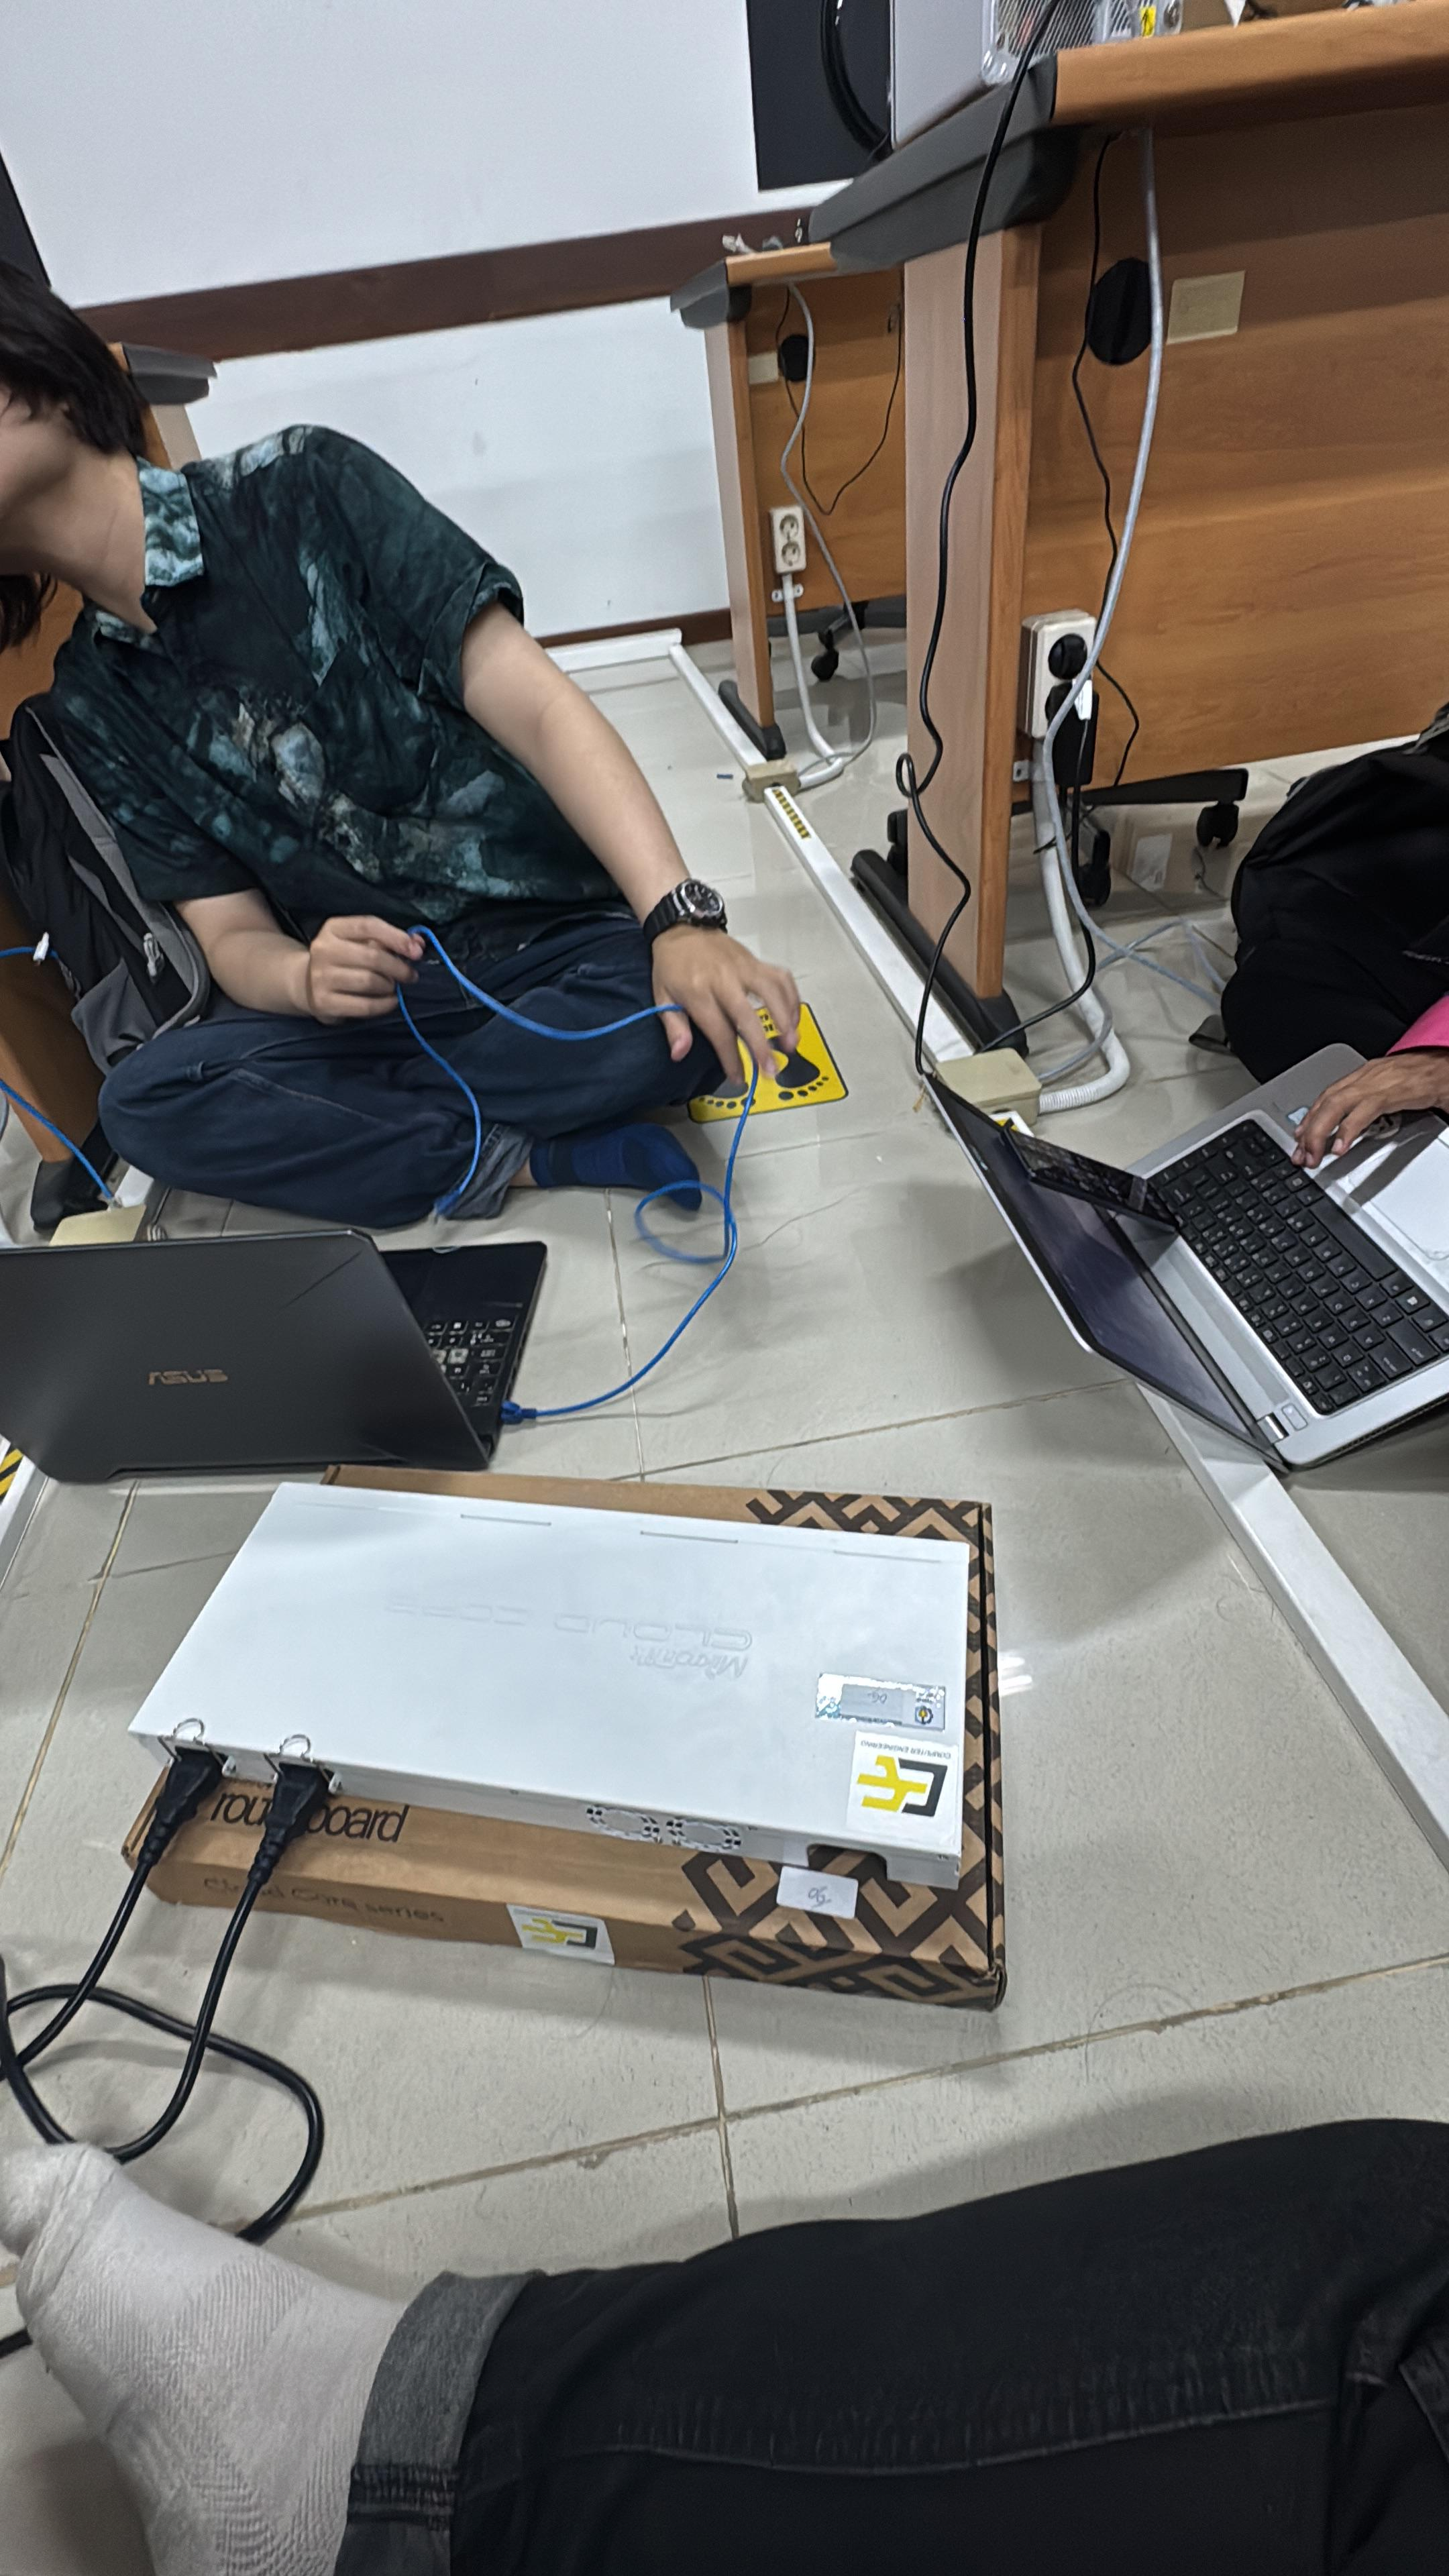
\includegraphics[width=0.65\linewidth]{image/dokum.jpg}
\end{figure}


\end{document}